\documentclass[12pt]{article}

\usepackage[slovene]{babel}
\usepackage[top=1in, bottom=1in, left=1in, right=1in]{geometry}
\usepackage{graphicx}
\usepackage{caption}
\usepackage[unicode]{hyperref}
\usepackage{tikz}
\usepackage{tikz-timing}
\usepackage{amsmath}
\usepackage[utf8]{inputenc}
\renewcommand{\contentsname}{Kazalo}
\renewcommand\listfigurename{Kazalo slik}
\renewcommand{\figurename}{Slika}
\usepackage{listingsutf8}

\begin{document}
\pagenumbering{gobble}
\linespread{1.25}
\begin{titlepage}
  \begin{center}
    
\includegraphics[height=2cm]{slike/vegova.png}\\
    \Huge
    \vspace*{6cm}
    Raziskovanje mej RISC-a\\
    \Large
    (računalništvo in informatika)\\
    Raziskovalna naloga\\
  \end{center}
  \vspace{8cm}
  \begin{tabular}{rl}
    Avtor: & Adrian Sebastian Šiška\\
    Mentor: & Aleš Volčini
  \end{tabular}
  \vspace{1cm}
  \begin{center}
    Ljubljana, marec 2022
  \end{center}
\end{titlepage}

\pagebreak
\pagenumbering{arabic}

\tableofcontents

\pagebreak

\listoffigures

\pagebreak

\section{Zahvala}
Zahvaljujem se vsem, ki so mi pomagali pri raziskovanju in pisanju.
Še posebej se zahvaljujem mentorju Alešu Volčiniju za podporo in potrpežljivost.
Zahvalil bi se tudi mojima prijateljema Oliverju Wagnerju (\url{oliwerix.com}) in Antonu L. Šijancu (\url{sijanec.eu}), ki sta s svojimi implementacijami emulatorja MUHI popestrila moje delo.

\pagebreak

\section{Povzetek}
V raziskovalni nalogi sem si zamislil novo RISC arhitekturo, imenovano MUHI (\textit{Minimal URISC hardware implementation}).
MUHI je enobitna, dvo-instrukcijska arhitektura.
Za njeno implementacijo sem raziskoval področje teorije izračunljivosti in arhitekture ostalih procesorjev.
Za testiranje delovanja sem sprogramiral emulator, za lažje pisanje programov pa sem pripravil tudi zbirnik in razbirnik.
Kot pomoč pri iskanju sestavljenih operacij sem napisal še program za iskanje kombinacij ukazov.
Implementacija je Turing-kompletna, kar sem dokazal tako, da sem napisal celični avtomat, ki izvaja pravilo 110.

Ključne besede: RISC, URISC, arhitektura procesorja, Univerzalen procesor, navidezna naprava, emulacija

\pagebreak

%% ANG ONLY DEU
% \section{Abstract}

\section{Uvod}
Procesorji so najpomembnejša komponenta v moderni zgradbi računalnika, kljub njihovi pomembnosti pa jih ljudje dandanes čedalje slabše razumejo.
Oblikovanje procesorjev smo prepustili relativno majhnim skupinam razvijalcev, z nizkonivojskimi jeziki pa se le še malokdo ukvarja.
To me čudi, saj vse od kar sem slišal za Intelov \textit{management engine} ne morem nehati razmišljati o mojem procesorju.
Spraševati sem se začel, kako lahko zares preverim, da management engine ni aktiven v mojem računalniku in ali lahko sploh zaupam svojemu procesorju.
To me je nekako pripeljalo do ideje, da naredim svoj procesor.
Tako sem si zamislil MUHI arhitekturo.

\subsection{Hipoteza}
V tej nalogi bom preveril resničnost sledeče hipoteze:
\begin{itemize}
  \item Moja lahkotna arhitektura imenovana MUHI je Turing-kompletna.
\end{itemize}

\section{Moja arhitektura}
\begin{center}
  %cd slike ; dot -O -Tpdf arhitektura.gv; cd ..
  \includegraphics[width=.5\linewidth]{slike/arhitektura.gv.pdf}
  \captionof{figure}{Shematika MUHI-ja}
\end{center}
Imenuje se \textit{Minimal URISC hardware implementation} oz.\ kratica MUHI.\@
\subsection{Kaj je URISC?}
% URGENTLY religate interesting stuff to the compiler
Kratica URISC pomeni \textit{ultimate reduced instruction set computer}, kar bi lahko v slovenščino prevedli kot \textit{računalnik z minimalno množico operacij}.
RISC arhitekture so v moderni praksi, boljše od CISC arhitektur, vsaj odkar pomnilnik ni več drag.
To nam dokazujejo moderni pametni telefoni, saj skoraj vsi delujejo na procesorjih vrste ARM.
To nam dokaže tudi najpopularnejši ustvarjalec CISC procesorjev, Intel, saj so dandanes njihovi procesorji interno zgrajeni iz tolmača in manjšega RISC procesorja.
Da arhitekturo označimo kot URISC, pa moramo iti še korak dlje in se znebiti vsek ukazov razen enega.
Zanimiva posledica tega je dejstvo, da lahko, ko pišemo strojno kodo, popolnoma spustimo polje z instrukcijo.
Tako ostanejo le še njeni argumenti.

V virih najdemo primere ukazov, ki so sami po sebi Turing-kompletni, npr.\ x86 mov ukaz\footnote{Stephen Dolan, mov is Turing-complete}.
Jaz sem se raje odločil za 2 instrukciji, ker se njuni rabi ne prekrivata zelo dosti, saj med drugim tudo operirata na različnih magnitudah količine podatkov.
Posledica dodatne instrukcije je lažje pisanje programov.
% Odločil sem se, da mi je težavnost pisanja programov brez prevajalnika pomembna, ker bi sicer ta naloga vzela še dosti več
Ker bi bilo opisovanje programiranja MUHI preveč obsežno, sem se odločil, da se bom v tej nalogi posvetil arhitekturi sami.

\subsection{Instrukcije}
%Obe instrukciji prejmeta 2 naslova iz rama\footnote{naslov ni nujno povezan z ramom, glej \textit{c16} instrukcijo} in en meta bit.
Obe instrukciji imata 3 argumente.
Prva dva argumenta sta registra, tretji pa je meta bit.
V moji izvedbi sem se odločil za 7-bitne\footnote{Ta izbira je arbitrarna, arhitektura podpira $n$ bitne naslove. 7-bitne sem izbral, ker je posledično dolžina ukaza v bitih strojne kode potenca števila 2.} pomnilniške naslove.
O organizaciji pomnilnika bom več povedal kasneje.

Strojna koda ukaza je sestavljena iz 1.\ naslova, 2.\ naslova, operacijske kode instrukcije in t. i. meta bita.

\begin{center}
  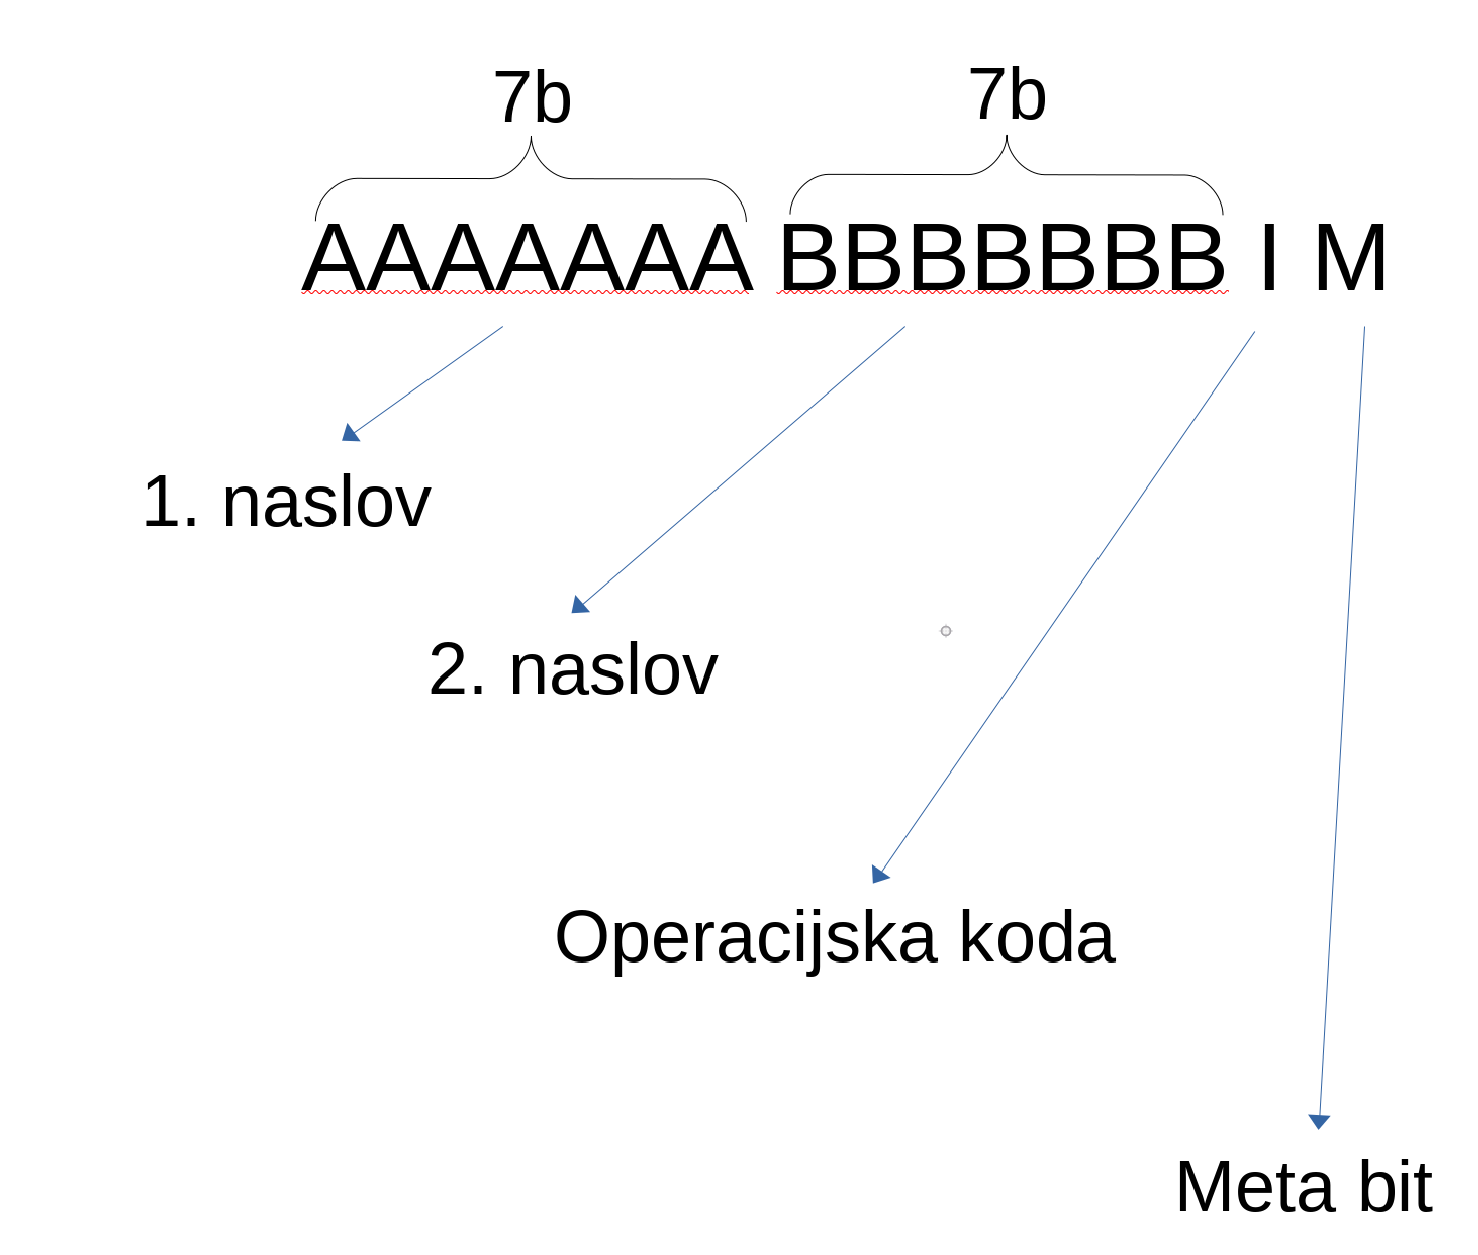
\includegraphics[width=.3\linewidth]{slike/zločinski_posnetek_zaslona.png}
  \captionof{figure}{Prikaz sestave strojne kode}
\end{center}

Meta bit je ostal zaradi poravnave dolžine ukaza na 2 bajta, s čimer je naredilo pisanje zbirnika in razbirnika nekoliko lažje.
Obe instrukciji se obnašata tako, da vzameta podatke iz 1.\ in 2.\ naslova ter rezultat shranita nazaj na 2.\ naslov.
\pagebreak
\subsubsection{Instrukcija ``c16''}

\begin{center}
  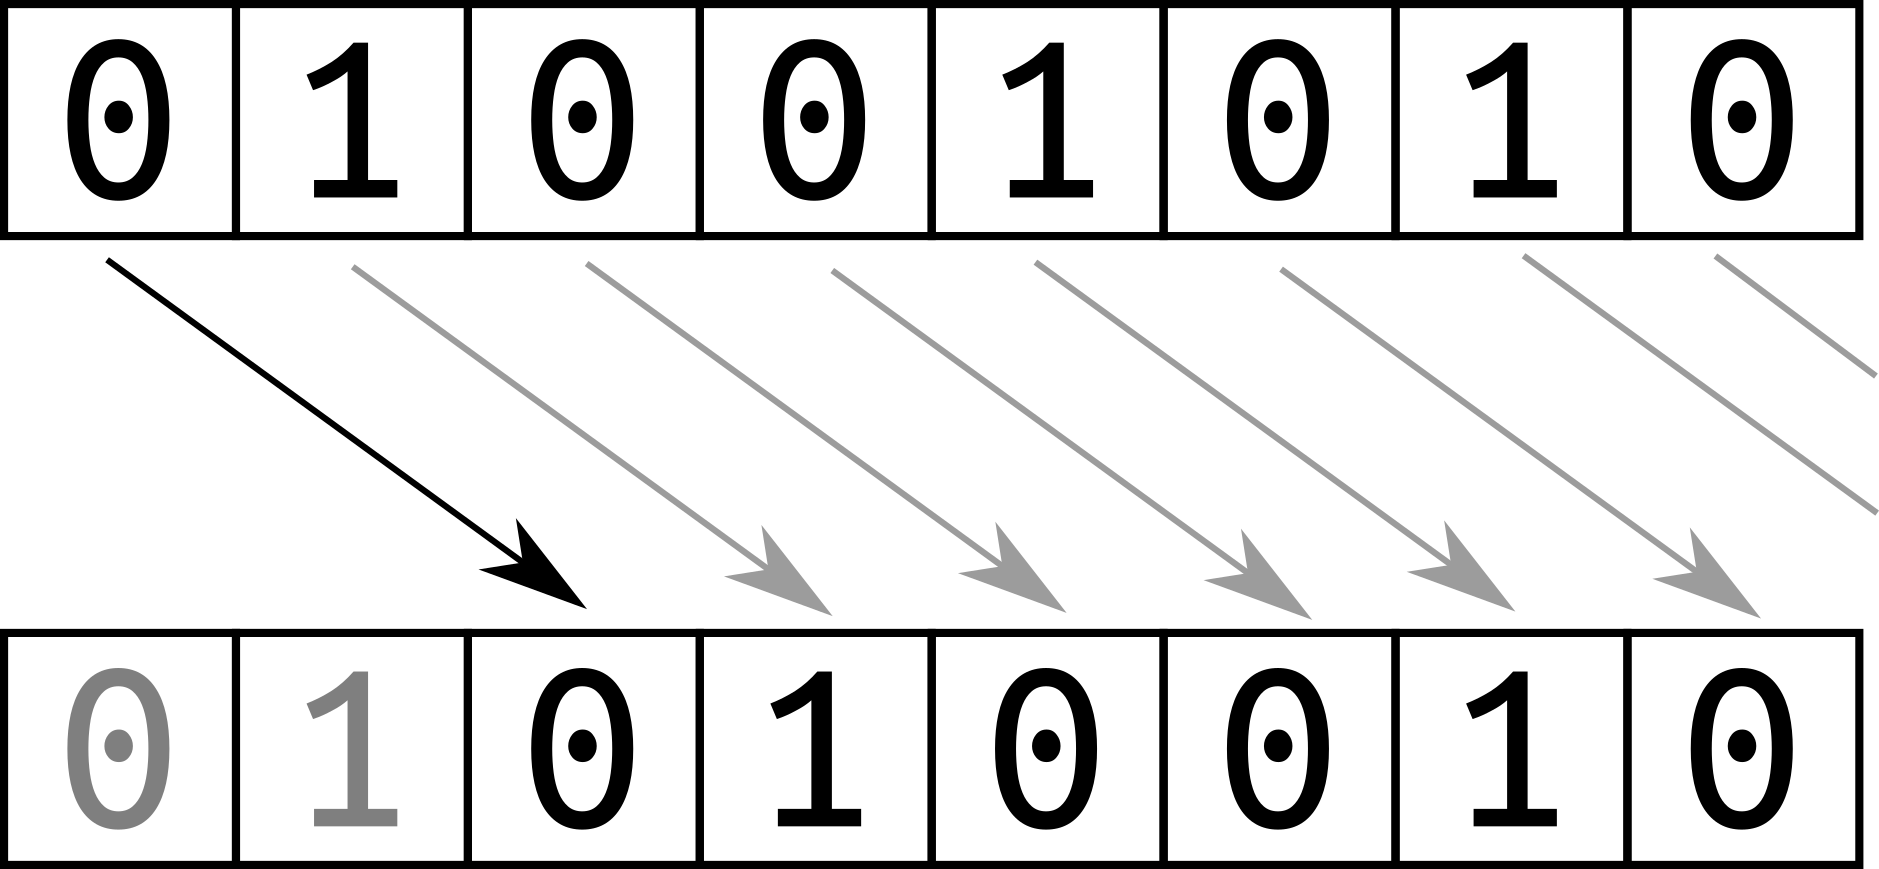
\includegraphics[width=.3\linewidth]{slike/predstavitev/copy.png}
  \captionof{figure}{Grafični prikaz c16 instrukcije}
\end{center}

To je 1.\ instrukcija, njena operacijska koda je $0$.
Njena notacija izhaja iz daljšega imena \textit{copy 16 bits}
Deluje tako, da od 1.\ podanega naslova 16 zaporednih registrov (\textit{oz.\ bitov}) prekopira v začasen pomnilnik, potem pa jih prekopira na 2.\ naslov.
Odločitev, da bo to 1.\ instrukcija, izhaja iz tega, da so same ničle v programu interpretirane kot ukaz brez posledic, kar je uporabno predvsem takrat, ko je potrebno z ničlami rabimo kaj poravnati na naslov, ki je nekaj mest nižje.
Na začetku je bila zasnovana skoraj kot jump instrukcija, saj z NANDom ni mogoče vseh bitov v programskem števcu hkrati spremeniti na željeno vrednost.
Posledica spremembe enega pa po enega bita v programskem števcu, bi bil skok takoj po 1.\ spremembi enega bita, saj kontrolna enota vedno preveri števec pred nalaganjem nove instrukcije.

Ko sem kasneje dodal še meta bit, sem se odločil, da se bo kopiranje ob nastavljenem meta bitu zgodilo iz programskega spomina.
S tem je nalaganje konstant, kot so nizi ali pa naslovi funkcij, postalo zelo preprosto in hitro.
Omejitev tega je, da sem uporabil 7 bitni naslov za pridobivanje podatkov iz programskega pomnilnika opisanega s 16 biti (uporabno je 128 bitov od 65536-ih).
Zaradi tega večina pomnilnika še vedno ni na voljo, kot rešitev temu pa sem se odločil, da sem uporabil skrite registre kot nastavitev strani programskega pomnilnika (\textit{memory page}).
Tako dobimo $2^{15}$ strani programskega pomnilnika.

Skriti registri namreč nastanejo kot stranski učinek omejitve velikosti naslova na 7 bitov.

Kaj se na primer zgodi, če pri kopiranju uporabimo zadnji register?
Ker instrukcija dostopa tudi do registrov nad 127, bi moral v tem primeru implementirati preliv (naslednji bi bil register 0) ali povsem ignorirati spreminjanje registrov od naslova 128 dalje.
Jaz sem se odločil za tretjo možnost -\ ostranjevanje pomnilnika.
Registre za zadnjim registrom sem najprej poimenoval \textit{skriti registri}.
Čeprav sem jih kasneje uporabil za ostranjevanje pomnilnika, njihovega poimenovanja še nisem zamenjal.
Ti registri so torej dostopni oz.\ v uporabi le, kadar kopiramo registre od 113 do 127.
Do njihove vsebine se da tako dostopati le s to instrukcijo, kar se mi ne zdi problem, saj se bodo strani pomnilnika menjavale le redko.

Torej se ukaz \verb|c16 0x22, 0x44, 0| prevede v \verb|0100010 1000100 0 0|, kar bi v programskem jeziku C tukaj lahko predstavili kot \\
\verb|int *a=0x22; int *b=0x44; *b=*a;*(b+1)=*(a+1)|\ldots \verb|*(b+15)=*(a+15)|.

Ker je instrukcija c16 edina instrukcija, ki je edina sposobna nastaviti programski števec na dano absolutno vrednost, sledi da mora biti tudi sposobna prekopirati vse bite programskega števca.

\subsubsection{Instrukcija ``Nox''}

\begin{center}
  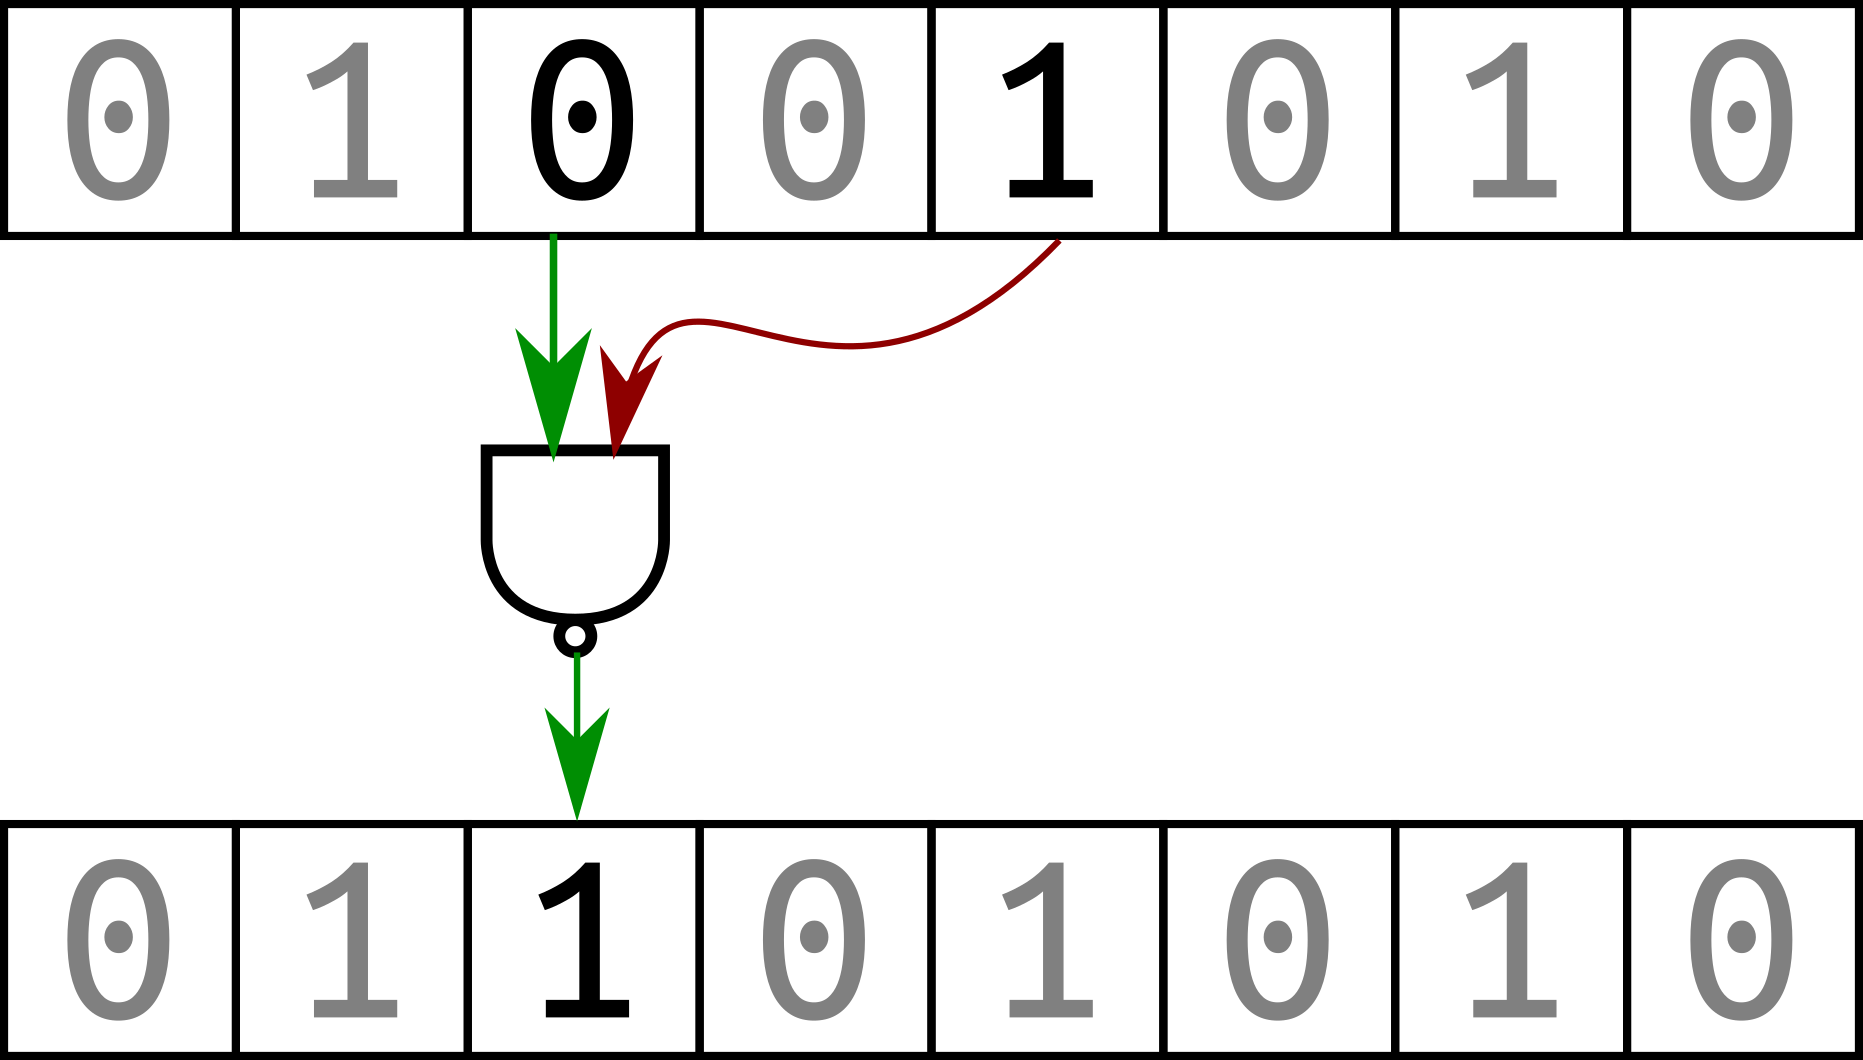
\includegraphics[width=.3\linewidth]{slike/predstavitev/nand.png}
  \captionof{figure}{Grafični prikaz nox instrukcije}
\end{center}

To je 2.\ instrukcija, njena operacijska koda je $1$.
Ime izhaja iz njenega kratkega opisa: \textit{NAND or XOR}.
Najprej sem poizkusil kot edini ukaz za manipulacijo bitov uporabiti le XOR.\
Vendar sem hitro ugotovil, da se samo z njo ne da rekonstuirati vseh ostalih logičnih vrat.
Zato sem se odločil še za najpogosteje izbrana univerzalna vrata NAND.\@

Ta so s seboj privlekla nove probleme; npr.\ pogojni skoki naprej so postali zelo dragi.
Programski števec bi sicer lahko bil viden samo instrukciji c16, vendar bi to preprečilo optimizacijo relativnih skokov na naslove, ki se od trenutnega razlikujejo v enem samem bitu (torej je odmik potenca števila 2).
Pogojni relativni skoki so razširitev zgornje ideje.
Ker vem, kje se nahaja trenuten ukaz, tudi vem, v kakšnem stanju je vsak bit programskega števca.
S kombiniranjem bita z vrednostjo 1 v programskem števcu in nekega podatka v ramu lahko skočimo nazaj samo takrat, ko je tudi podatek v ramu enica.
Pogojen skok naprej ni izvedljiv na tak način, saj bi na mestu bita v programskem števcu, ki ga želimo pogojno povečati, morala biti ničla.
Operacija NAND v primeru, da, je katerikoli izmed argumentov 0, vedno da rezultat 1, kar pomeni, da naše \textit{pogoj} iz pogojnega skoka ni bil upoštevan.

Zaradi dragih skokov in lahke ponastavitve celice na 0, sem se odločil, da dodam še XOR.\@
Par vrat sem kombiniral v eno instrukcijo, kjer meta bit izbira med njima.

\begin{displaymath}
  f(A,B,M) =
  \begin{cases}
    NAND(*A, *B) \rightarrow *B & M=0\\
    XOR(*A, *B) \rightarrow *B & M=1
  \end{cases}
\end{displaymath}
$*A$ pomeni priklic in zapis na register z naslovom $A$

Če zgornje izrazimo z logično notacijo, dobimo:
\begin{displaymath}
  \overline{(AB)}(A+B+\overline{M})
\end{displaymath}

Torej se ukaz \verb|Nox 0x15, 0x53, 0| prevede v \verb|0010101 1010011 1 0|, kar bi v programskem jeziku C tukaj lahko predstavili kot \verb|int *a=0x15;int *b=0x53;*b=NAND(*a,*b)|.

\pagebreak
\subsection{Enobitni registri (\textit{podatkovni pomnilnik})}
% vsi registri so eneaki, samo eni so bol enaki

\begin{center}
  
\includegraphics[width=\linewidth]{slike/predstavitev/reg.png}
  \captionof{figure}{Grafični prikaz registrov}
\end{center}

Ram sem si zamislil, kot \textit{trak} enobitnih registrov.
Zaradi preprostosti je programski števec preslikan čez prvih 16 registrov, da lahko z njim operira tudi instrukcija \textit{Nox}.
Za njim sledijo štirje biti vhodno-izhodnega (I/O) naslovnega prostora.
Več o njih bom povedal kasneje.
Število vseh registrov je funkcija dolžine naslova rama in velikosti programskega števca.
Za računanje dolžine traka registrov sem pripravil preprosto formulo.
$F(N,P)$, v mojem primeru $F(7,16)$, izračuna število registrov, ki jih imam na razpolago, pri danem N in P.
\begin{center}
  \begin{displaymath}
    F(N,P)=2^{N}+P-1
  \end{displaymath}
  $F(N,P)$ je število registrov, $N$ je dolžina binarnega naslova, $P$ je dolžina programskega števca
\end{center}

\subsection{Programski pomnilnik}
Programski pomnilnik je organiziran v šestnajst-bitne besede.
Njegova velikost znaša 65536 besed oz. 131072 bytov.
Vsebuje lahko instrukcije ali konstante.
Programski števec vsebuje naslov instrukcije, ki se bo ob naslednjem ciklu izvedla.
Edini način za branje iz njega je z c16 instrukcijo, za pisanje vanj pa trenutno še ni mehanizma.


\subsection{Komunikacija z zunanjim svetom}
Za izvedbo vhodno-izhodnih operacij se odločil, da bom implementirati svojo 4-žično komunikacijo.
Ta lahko asinhrono prenaša informacije bit za bitom.
Asinhronost je pomembna lastnost, saj arhitektura nima prostora za začasen pomnilnik, ki bi shranjeval podatke za čas, ko bi se program lahko začel z njimi ukvarjati.

Po drugi strani bi prekinitve (interrupts) dodale ogromno kompleksnosti, kot npr.\ najmanj 16 dodatnih registrov, instrukcijo za branje z njih, možnost spreminjanja registrov, ki ni posledica nekega ukaza itd.
Lepa lastnost štirižičnega protokola je tudi, da se dve napravi z lahkoto skupaj poveže, saj moramo le izhode iz ene priklopti v vhode druge.
\begin{center}
  \begin{tabular}{ccc}
    $A_{OUT}  $ & \texttiming{LHHHLLLLLL} & $B_{IN}$\\
    $A_{OUT_A}$ & \texttiming{LLHZLLLLLL} & $B_{IN_A}$\\
    $A_{IN}   $ & \texttiming{LLLLLHHHHL} & $B_{OUT}$\\
    $A_{IN_A} $ & \texttiming{LLLLLLHZLL} & $B_{OUT_A}$
  \end{tabular}\footnote{modra črta na sredini prikaže stanje, kjer ena naprava drži signal pri logični enici, druga naprava pa ga poizkuša nastaviti na ničlo}

  \text{Primer pošiljanja enice od A do B in od B do A}
\end{center}
Za pošiljanje informacij najprej počakamo, da je $OUT_{A}$ dovoljen, torej 0.
Nato lahko pišemo, kar hočemo, v $OUT$, dokler ne želimo vrednosti \textit{oddati}, kar naredimo s tako, da napišemo enico na $OUT_{A}$.

Za prejemanje informacij je postopek podoben.
Začnemo s preverjanjem $IN_{A}$, kot da bi gledali nabiralnik, če nam je poštar kaj prinesel.
Čim dobimo napisano enico, smemo interpretirati karkoli je trenutno v $IN$, kot podatke.
Da dobimo naslednji znak, priklopimo pulldown upor na $IN_{A}$.
To druga naprava zazna in čim prej spusti $IN_{A}$ na 0.


\section{Izdelava}
Najprej sem se odločil da bom potreboval okolje, kjer bi lahko testiral arhitekturo, spremembe in moje programe.
Zato sem se lotil pisanja virtualnega stroja.
Ker je brez preizkusov težko vedeti, ali stroj pravilno deluje, sem začel delo na zbirniku, da mi ne bi bilo več treba na roke pisati enic in ničel.
Seveda je izdelava zbirnika tudi težka, zato sem razvil še razbirnik, s katerim preverim delovanje zbirnika.
Izdelava le tega je bila nekoliko lažja, kljub temu pa sem našel večjo napako pri dekodiranju ukazov šele po nekaj dneh.

Virtualni stroj, zbirnik in razbirnik sem napisal v programskem jeziku python.
\subsection{Zbirnik (assembler)}
Glej prilogo \textit{asm.py}.

\begin{center}
  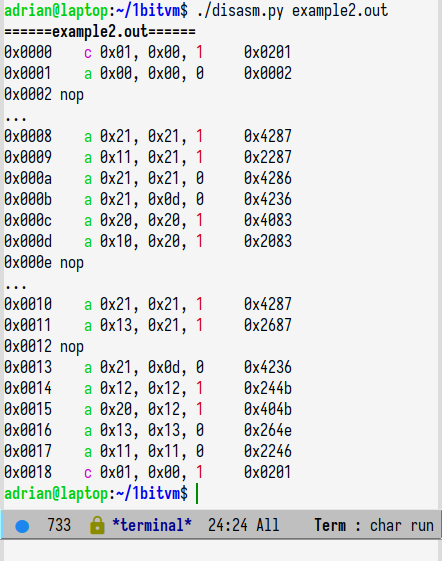
\includegraphics[width=.3\linewidth]{slike/razbirnik.png}
  \captionof{figure}{Grafični prikaz nox instrukcije}
\end{center}

Najprej celotno datoteko podamo NASMovemu preprocesorju.\footnote{NASM (\textit{The Netwide Assembler}) je popularen x86 zbirnik, ki mi služi le kot preprocesor.}
Preprocessor skrbi za dodajanje večih datotek skupaj in razširjanje makrov ter definicij.
Ker moramo zaradi oblike zbirnega jezika ohraniti vrstice iz izvorne kote, C-jev preprocesor ni primeren.

Potem za vsako vrstico v datoteki naredimo naslednje:
\begin{itemize}
  \item preiščemo vrstico za par ``$<py>$'' simbolov, ki tvorita python blok.
  Vsaka uporabnikova konstanta je tako ali tako interpretirana kot izraz v pythonu, vendar nastane problem, ko želimo interpretirati izraze, ki vsebujejo vejice.
  Vejice so namreč ločilo med polji, zato moj preprost program nareže en pythonov izraz na več majhnih delov, ki sami po sebi niso več veljavni.
  \item Na koncu vse py bloke zamenjamo z njigovimi izračunanimi vrednostmi v vrstici.
  \item Nato klasificiramo vsako vrstico v eno izmed petih možnih vrst.
  \begin{itemize}
    \item Komentar ali prazna vrstica, ki jo lahko varno spustimo,
    \item Surovi binarni podatki, ki jih direktno zapišemo v datoteko,
    \item Premik v programu: premaknemo mesto pisanja in nadaljujemo,
    \item Instrukcija v procesorju, ki jo dekodiramo, izračunamo njene argumente in zapišemo,
    \item Naslov, katerega pozicijo si zapomnimo, da bomo kasneje lahko omenjali predmet pred katerim stoji.
  \end{itemize}
\end{itemize}

\subsection{Razbirnik (Dissasembler)}
Glej prilogo \textit{disasm.py}.

\begin{center}
  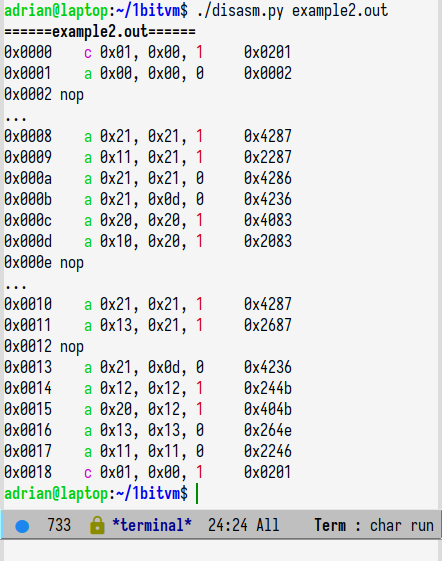
\includegraphics[width=.3\linewidth]{slike/razbirnik.png}
  \captionof{figure}{Primer uporabe razbirnika}
\end{center}
Med izdelavo delujočega zbirnika sem naletel na nekaj problemov, zato sem z malo pomoči soseda Oliverja napisal še manjši program, ki se sprehodi čez datoteko in jo interpretira v instrukcije in njene argumente.
Izpiše nam naslov, na katerem se ukaz nahaja, ukaz sam, meta bit in še šestnajstiški prikaz tega ukaza, saj ne loči med podatki in ukazi.

\subsection{Iskanje ukazov s surovo silo}
Glej prilogo \textit{gate-bf}.

\begin{center}
  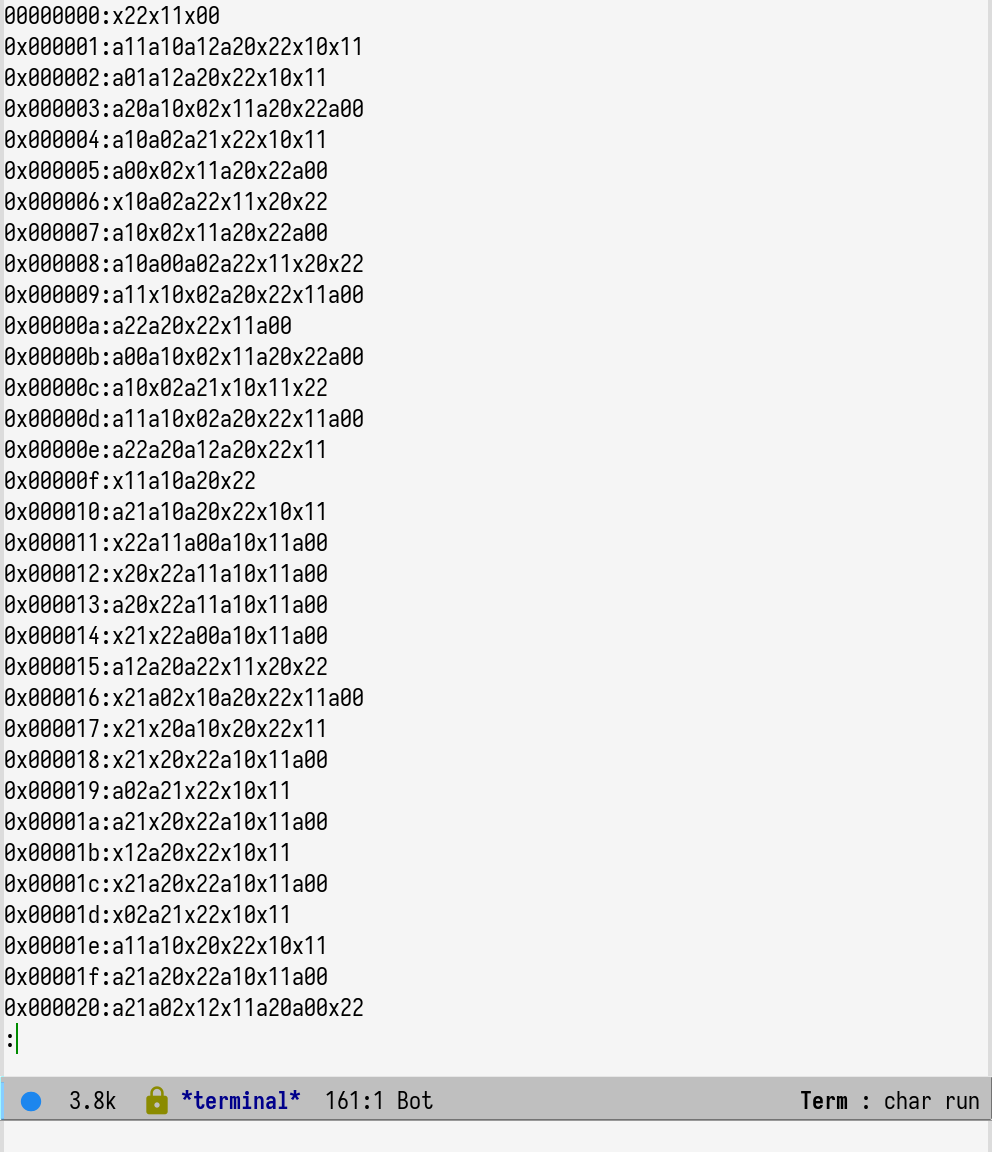
\includegraphics[width=.3\linewidth]{slike/predstavitev/gate-bf.png}
  \captionof{figure}{Prikaz tabele z vsemi možnimi rezultati}
\end{center}

Pisanje makrov, kot so \texttt{add} je za človeka zaradi nepreglednosti težko opravilo.
Seveda se da poiskati kombinacijo NAND-ov in XOR-ov, ki bi mi vrnila seštevek dveh številk, vendar ne morem biti prepričan, da sem res našel najkrajši način za to.
Zato sem napisal program, ki najde najkrajše kombinacije ukazov namesto mene in jih zapiše v tabelo.
V taki tabeli poiščemo mesto s številskim opisom našega problema in prepišemo zaporedje ukazov, ki ta problem reši.
Ideja je v tem, da za vsak možen vhod v $n$ celic preizkusimo vse možne ukaze, in gledamo, kdaj dobimo nov rezultat.
Ko dobimo kaj novega, lahko preprosto ponovimo postopek.
Tako lahko generiramo tabelo rezultatov glede na vse možne vhode.

Prva implementacija tega programa je bila napisana v pythonu in bi po mojih ocenah trajalo nekaj tednov, da bi z njo dobil popolno tabelo vseh možnih rezultatov.
Zato sem prepisal cel program v C in z uporabo več niti hkrati skrajšal čas iskanja na 3 sekunde.

\section{Virtualna implementacija}
Glej prilogo \textit{main.py}.

Da zares lahko pokažemo delovanje naprave, moramo nekako prikazati kako deluje.
To na najlažji način danes dosežemo z implementacijo v virtualnem okolju.
Zato sem se lotil pisanja virtualne naprave v pythonu.
Virtualna naprava ima vse lastnosti prej opisane arhitekture.
Ima implementirano konzolo, v razhroščevalnem načinu pa tudi vpogled v notranje stanje.
Tako lahko preko terminala z navidezno napravo tudi komuniciramo.
To lahko najlažje vidimo pri primeru št. 1 (priloga), kjer naprava izpiše ``Zivjo'', ali v primeru št. 2, kjer nam naprava vrne nazaj vsak bit, ki ga prejme.

\subsection{Celični avtomat}

\begin{center}
  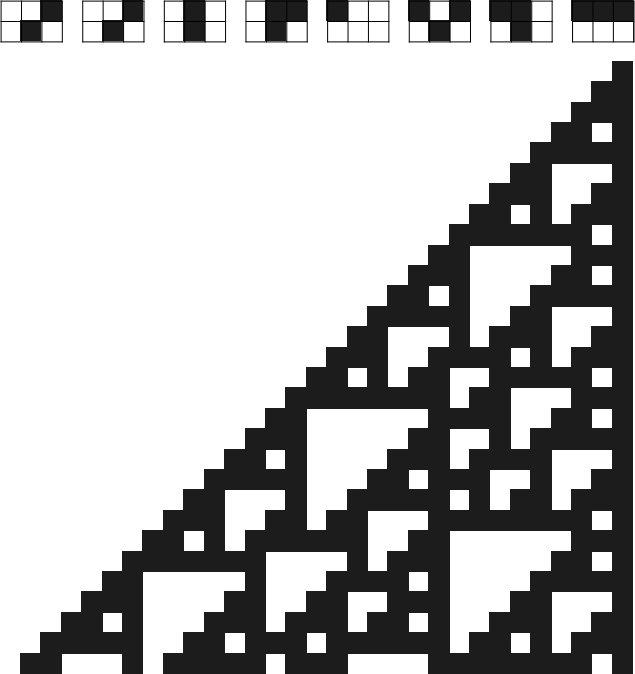
\includegraphics[width=.3\linewidth]{slike/predstavitev/pravilo 110.png}
  \captionof{figure}{Pravilo 110}
\end{center}
\begin{center}
  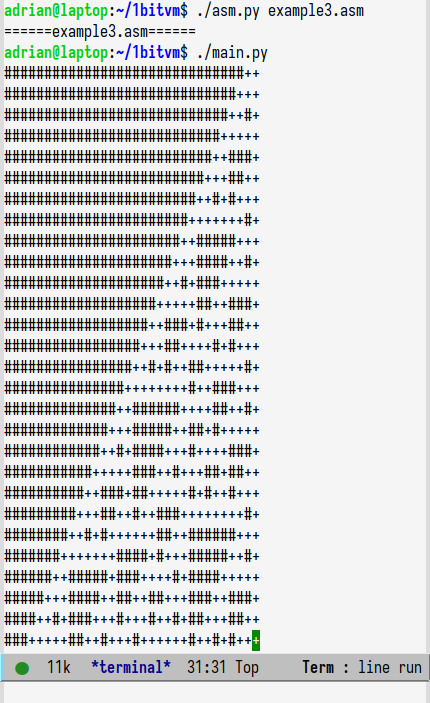
\includegraphics[width=.3\linewidth]{slike/pravilo110.png}
  \captionof{figure}{Prikaz delovanja celičnega avtomata na MUHI arhitekturi.}
\end{center}
Za dokazovanje, da je arhitektura MUHI turing-kompletna, sem izbral emulacijo drugega turing-kompletnega sistema.
Eden izmed najbolj preprostih, čeprav še vedno dovolj kompleksnih, da je univerzalen, je Celični avtomat s pravilom 110. [$3$]
Seveda ne morem implementirati neskončno dolgega enodimenzionalnega traka, na katerem bi simuliral izvajanje tega pravila, lahko pa pokažem, da bi se to dalo implementirati, če bi moja naprava imela neskončno rama.

\section{Zaključek}
\subsection{Hipoteza}
\begin{itemize}
  \item Moja lahkotna arhitektura imenovana MUHI je Turing complete.
  Hipoteza potrjena, saj lahko popolnoma emulira sistem, za katerega je že bilo dokazano, da je turing-kompleten.
\end{itemize}

\section{Priloge}

Vse priloge in izvorna koda so dosegljive na \url{https://github.com/adimineman/raziskovalna} in so licencirane z odprtokodno licenco.

\lstset{
  basicstyle=\tiny,
  breaklines=true,
  frame=single,
  stepnumber=5,
}
\lstdefinestyle{py}{
  language=Python,
}

\lstdefinestyle{asm}{
  language=[x86masm]Assembler,
  morekeywords={copy, nand, xor, x, a, c},
}
\lstdefinestyle{cst}{
  language=C,
}

\lstinputlisting[style=py,caption=asm.py]{1bitvm/asm.py}
\lstinputlisting[style=py,caption=disasm.py]{1bitvm/disasm.py}
\lstinputlisting[style=asm,caption=example.asm]{1bitvm/example.asm}
\lstinputlisting[style=asm,caption=example2.asm]{1bitvm/example2.asm}
\lstinputlisting[style=asm,caption=example3.asm]{1bitvm/example3.asm}
\lstinputlisting[style=asm,caption=std.asm]{1bitvm/std.asm}
\lstinputlisting[style=py,caption=main.py]{1bitvm/main.py}
%\lstinputlisting[caption=Primer razporeditve pomnilnika]{1bitvm/mem}
\lstinputlisting[style=py,caption=oneb\_vm.py]{1bitvm/main.py}
\lstinputlisting[style=cst,caption=gate-bf]{gate-bf/main.c}

\pagebreak
\section{Viri in literatura}
$[1]$ Andreas Abel, upops.info: Characterizing Latency, Throughput, and Port Usage of Instructions on Intel Microarchitectures, ACM, 2019, dosegljivo: \url{https://uops.info/} [23.3.2022]\\
$[2]$ Crystal Chen, RISC architecture, 2000, dosegljivo: \url{https://cs.stanford.edu/people/eroberts/courses/soco/projects/risc/risccisc/} [23.3.2022]\\
$[3]$ Matthew Cook, Universality in Elementary Cellular Automata, Department of Computation and Neural Systems, 2004, dosegljivo: \url{https://wpmedia.wolfram.com/uploads/sites/13/2018/02/15-1-1.pdf} [23.3.2022]\\
$[4]$ Stephen Dolan, mov is Turing-complete, Computer Laboratory, University of Cambridge, 2013, dosegljivo: \url{https://harrisonwl.github.io/assets/courses/malware/spring2017/papers/mov-is-turing-complete.pdf} [19.4.2022]\\

% \pagebreak
% \section{Viri slik}
\end{document}
